\textbf{Example}

Let $N=4$, $H=[2,4,3,5]$, $Q=2$, and $R=[2,3]$.

The grader calls \texttt{minimum\_costs([2, 4, 3,
5], [0, 1], [2, 3])}.

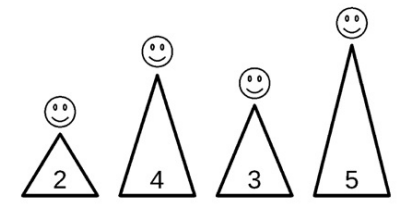
\includegraphics{1.png}


The meeting $j=0$ has $L_j=0$ and $R_j=2$, so will be attended by the people living on
the mountains $0$, $1$, and $2$. If the mountain $0$ is chosen as the meeting place, the cost of
the meeting $0$ is calculated as follows:
\begin{itemize}
    \item The cost of the participant from the mountain $0$ is $\max(H_0)=2$.
    \item The cost of the participant from the mountain $1$ is $\max(H_0, H_1)=4$.
    \item The cost of the participant from the mountain $2$ is $\max(H_0, H_1, H_2)=4$.
    \item Therefore, the cost of the meeting $0$ is $2 + 4 + 4 = 10$.

\end{itemize}
It is impossible to hold the meeting $0$ at a lower cost, so the minimum cost of the
meeting $0$ is $10$.

The meeting $j=1$ has $L_j = 1$ and $R_j=3$, so will be attended by the people living on
the mountains $1$, $2$, and $3$. If the mountain $2$ is chosen as the meeting place, the cost of
the meeting $1$ is calculated as follows:

\begin{itemize}
    \item The cost of the participant from the mountain $1$ is $\max(H_1, H_2)=4$.
\item The cost of the participant from the mountain $2$ is $\max(H_2)=3$.
\item The cost of the participant from the mountain $3$ is $\max(H_2, H_3)=5$.
\item Therefore, the cost of the meeting $1$ is $4 + 3 + 5 = 12$.

\end{itemize}


It is impossible to hold the meeting $1$ at a lower cost, so the minimum cost of the
meeting $1$ is $12$.

The files sample-01-in.txt and sample-01-out.txt in the zipped attachment
package correspond to this example. Other sample inputs/outputs are also available in
the package.